\section{addition}






\subsection{Runtime}

\begin{figure}
\centering
% Requires \usepackage{graphicx}
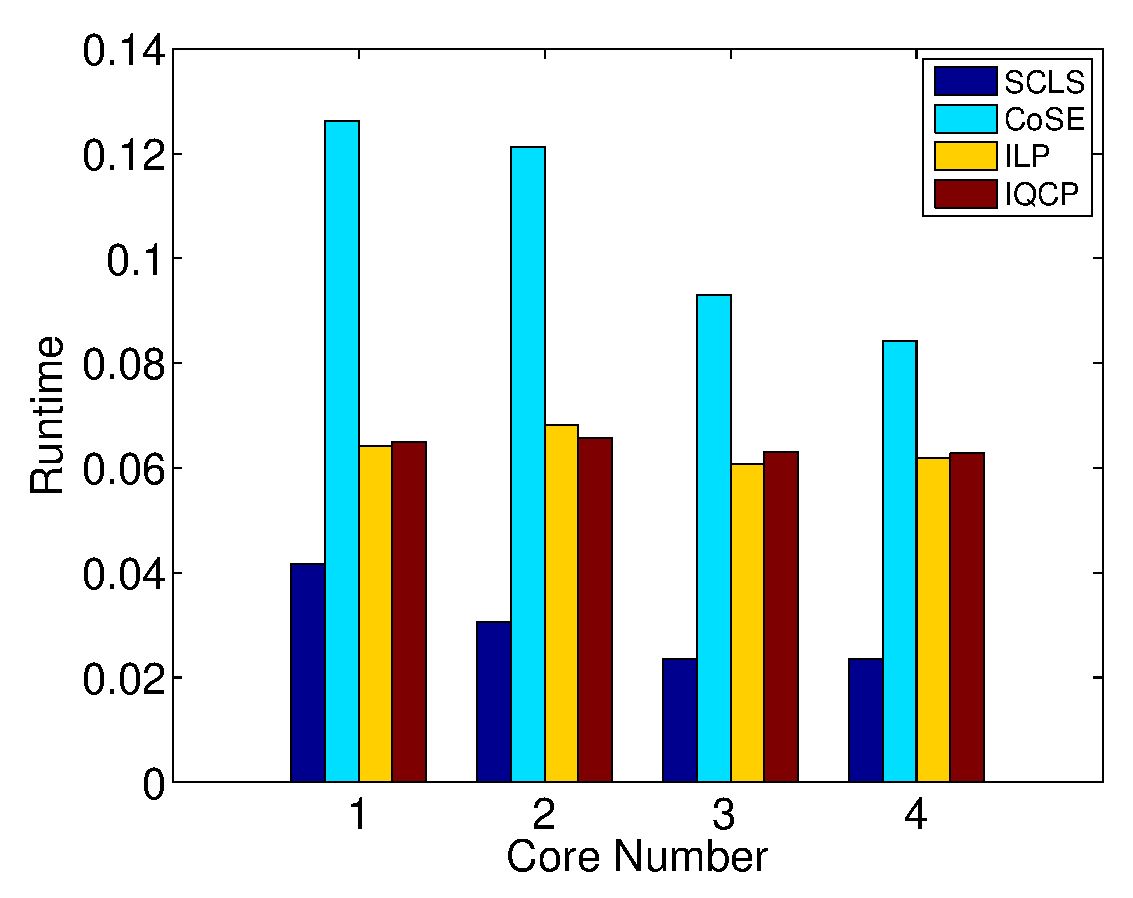
\includegraphics[width=2.35in]{franz/Runtime_NoKSP}\\
\caption{Runtime without KSP algorithm}\label{fig:Runtime_NoKSP}
\end{figure}

Runtime of CoSE is high than ILP and IQP as shown in Fig.\ref{fig:normalization runtime}.\ref{fig:Runtime_NoKSP} because the CoSE find the path AP with more time consumption when conflicting SRLG set is relatively large-scale. Suppose $r_i(1\leq i\leq \lambda)$ is the ith SRLG of conflicting SRLG set from algorithm CoSE, $\lambda$ is elements number of  conflicting SRLG set, $r_c$ is the largest edges number of all risk $r_i$, some edge which do not belong any risk equal a sole risk $r$. When CoSE obtain a conflicting SRLG set and divided and divided original problem by this set as our proposed parallel structure as illustrated in Fig.\ref{fig:DividedConquer}, there are $\lambda$ subproblems, $\mathcal{P}(\emptyset,\{r_1\}),\mathcal{P}(\{r_1\},\{r_2\}),\cdots ,\mathcal{P}(\{r_1,r_2,\cdots ,{r_{ \mathbb{\lambda} -1}}\},\{r_{ \mathbb{\lambda} }\})$ execute in parallel to obtain optimal solution. The time complexity of algorithm CoSE is dependent on the highest time complexity of finding path $AP$ of $\lambda$ subproblems. Subproblem of the highest time complexity is $\mathcal{P}(\{r_1,r_2,\cdots ,{r_{| \mathbb{\lambda} |-1}}\},\{r_{| \mathbb{\lambda} |}\})$, whose time complexity is $O(r_c^{\lambda-1}\times (\lambda-1) !\times|\mathbb{E}|\times log(|\mathbb{V}|))$. Finding $AP$ must pass one edge from every risk $r_i(1\leq i\leq (\lambda-1))$ in subproblem $\mathcal{P}(\{r_1,r_2,\cdots ,{r_{| \mathbb{\lambda} |-1}}\},\{r_{| \mathbb{\lambda} |}\})$. This is equivalent to a NP-complete problem which is shortest path visiting all nodes of specified nodes set $\mathbb{S}$, whose time complexity is $O(|\mathbb{S}| !\times|\mathbb{E}|\times log(|\mathbb{V}|))$. Therefore, there are at most $r_c^{\lambda-1}$ enumeration combination about specific nodes set in subproblem $\mathcal{P}(\{r_1,r_2,\cdots ,{r_{| \mathbb{\lambda} |-1}}\},\{r_{| \mathbb{\lambda} |}\})$ and every specific nodes set just have $\lambda-1$ nodes. Besides, our algorithm just have one specific nodes set and the size of this set is $|\mathbb{T}|-1$, Therefore, time complexity of our algorithm is $O({(|\mathbb{T}|-1)}!\times |\mathbb{E}|\times log(|\mathbb{V}|))$. Every edge of SRLG conflicting link set of our algorithm is of equivalent one or more SRLG so that in most situation $\mathbb{T}\leq \lambda$.

When $|\mathbb{T}|$ is small number, the time complexity of our algorithm is approximate to polynomial time complexity. so we emphasize that we should gain a small scale of $\mathbb{T}$.

The highest runtime is from algorithm KSP in Fig.\ref{fig:normalization runtime}, even though time complexity of the standard KSP algorithm is $O(\mathbb{V}+\mathbb{E}\times log(\mathbb{E})+k)$\cite{eppstein1998finding}, the algorithm KSP do not determine which k-shortest path is the minimum $AP$ which is SRLG-disjoint with $BP$.
The KSP algorithm just enumerate the all nodes so that determine which k-shortest path, the time complexity of algorithm of enumeration operation is $O(2^\mathbb{E})$(There are multiple edges between two adjacent nodes). All in all, time complexity of KSP algorithm solving SRLG-disjoint problem is $O(2^\mathbb{E}\times (\mathbb{V}+\mathbb{E}\times log(\mathbb{E})+k))$, these situation like in Fig.\ref{KSPproblem}.







